\section{Introduction to downfolding the many electron problem}

In multiscale modeling of many-particle systems, the effective Hamiltonian (or Lagrangian) is one of the most core concepts. 
The effective Hamiltonian dictates the behavior of the system on a coarse-grained level, where 'sub-grid' effects are folded into the parameters and form of the effective Hamiltonian. 
Fundamental concepts in condensed matter physics can be viewed as statements about the behavior of the effective Hamiltonian as the length scales change. 
For example, in a scale invariant system the effective Hamiltonian does not change as the length scale changes \HJC{eff Ham  changes but its "form" doesnt change? Would that be more technically correct?}, while a system with emergent physics has a different form of effective Hamiltonian when described at different length scales\lucas{I'm nervous about saying these things; please take a look and comment.}. 
These principles form the basis of the renormalization group\cite{Wilson}.
A major goal in condensed matter physics is to determine what effective Hamiltonians apply to different physical situations, in particular quantum effective Hamiltonians, which lead to large-scale emergent quantum behavior. 

The dominant effective model for quantum particles in condensed systems is band structure, and for metals, Fermi liquid theory. 
However, a major challenge is how this paradigm should be altered when it is no longer a good description of the physical system.
A famous example of this is the high-T$_c$ cuprates and other transition metal oxides, which do not appear to be well-described by these simple and classic effective Hamiltonians. 
For these systems, many models have been proposed, such as the Hubbard~\cite{Hubbard}, t-J~\cite{tJSpalek} and Heisenberg models.
While these models have been extensively studied analytically and numerically, and have significantly enhanced our understanding of the physics of correlated electrons, their effectiveness for describing a real complex system of interest is often unclear. 
At the same time, more complex effective models can be commensurately more difficult to solve, so the desire but also to find an accurate effective model that is tractable. 



\begin{figure}
\centering
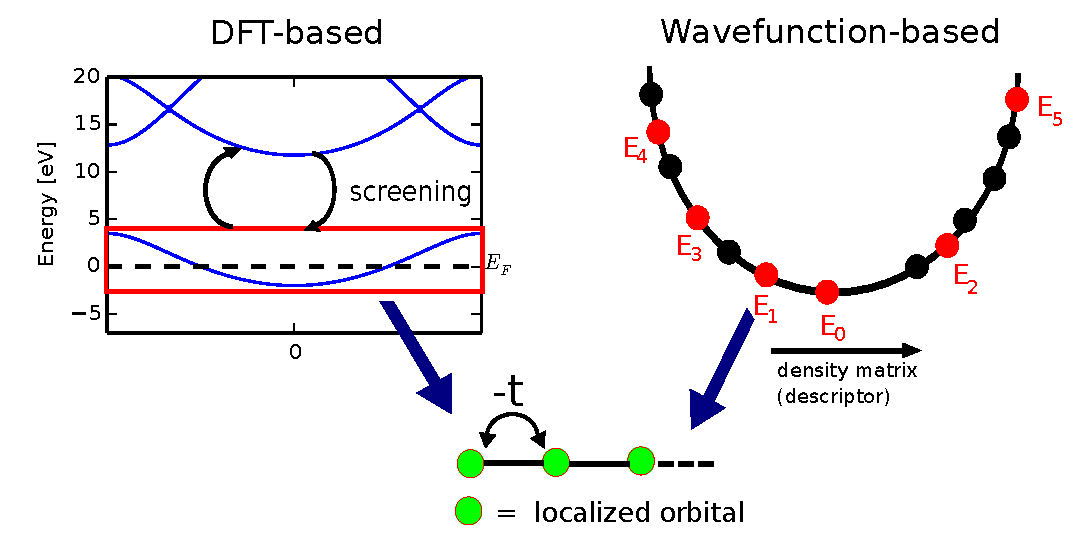
\includegraphics[width=1\linewidth]{./Figures/figure1.eps}
\caption{Schematics for downfolding a simple ab-initio system (here the hydrogen chain) in DFT based methods (left) and the wave function based AIDMD (right). 
Localized one particle functions are constructed in both methods and serve as the one body space for the model Hamiltonian. 
The DFT based methods use Kohn Sham orbitals and screening models to estimate the interactions. 
AIDMD uses a database of low energy all electron many-body wave functions ($\psi_i$). 
This "low energy basin" (shown abstractly in the space of descriptors) need not consist of exact eigenstates ($E_i$).\lucas{The energy should be a linear function of the density matrix!}}
\label{fig:lowenergybasin_schematic}
\end{figure}	


To address the need for a link between {\it ab-initio} electron-level  models and larger scale models, downfolding has most commonly been carried out using approaches based on density functional theory (DFT). 
The kinetic part is obtained from a standard DFT calculation which is projected onto localized Wannier functions and gives an estimate of the effective hoppings of the lattice model~\cite{Pavirini}. 
Then, to estimate the interactions, one assumes a model of screening of the Coulomb interactions based on constrained DFT, RPA, or some other method. 
Since effects of interactions between the orbitals of interest have already been accounted for by DFT, a double counting correction is required to obtain the final downfolded Hamiltonian. \lucas{There is a claim of no double-counting for GW-type fitting; can someone comment on this?}
The approach has been developed and widely applied~\cite{};\lucas{citations} but remains an active area of research~\cite{Haule_doublecounting}.
There are other downfolding approaches that include the traditional Lowdin method, coupled to a stochastic approach~\cite{Tenno,Zhou_Ceperley} and the related method of canonical transformations~\cite{White_CT, Yanai_CT}. 
While they have many advantages, all of these methods suffer from a lack of internal checks on the quality of the resultant model--it is typically not possible to know if a given model {\it ansatz} was a good guess or not. \lucas{Check this..} \HJC{I think CT may have internal checks of some sort.. need to check} 

The situation described above stands in contrast to the derivation of effective classical models. 
For concreteness, let us discuss classical force fields computed from {\it ab initio} electronic structure calculations. 
Typically, a data set is generated using an {\it ab initio} calculation in which the positions of the atoms and molecules are varied, creating a set of positions and energies. 
The parameters in the force field {\it ansatz} are varied to obtain a best-fit classical model.
Then, using standard statistical tools, it is possible to assess how well the fit reproduces the {\it ab initio} data within the calculation, without appealing to experiment. 
While translating that error to error in properties is not a trivial task\lucas{citations}, this approach has the important advantage that in the limit of a high quality fit and high quality {\it ab initio} results, the resultant model is predictive.

Na\"ively, one might think to reconcile the fitting approach used in classical force fields with quantum models by matching eigenstates between the (now quantum) model and {\it ab initio} systems, varying the model parameters until the eigenstates match. 
However, this strategy does not work well in practice because it is often not possible to obtain exact eigenstates for either the model or the {\it ab initio} system.
To resolve this, we develop a general theory for generating effective quantum models that is exact when the wave functions are sampled from the manifold of low-energy states, and is a good approximation when the sampled manifold is parallel to that manifold in the model space. 
Because this method is based on fitting the energy functional, 
We will show the practical application of this theory using both exact solutions and {\it ab initio} quantum Monte Carlo to derive several different quantum models.
\HJC{We should define our acronym "AIDMD" in the above para}


\lucas{I think the bulk of this could go in Section 4--what use these models will have.}
\HJC{Yes, I agree the bulk should go but we should devote two lines here also} 
The endeavor we pursue here is to develop a multi-scale approach in which the effective interactions between quasiparticles (such as dressed electrons) are determined after an \textit{ab-initio} simulation (but not necessarily exact solution) of the continuum Schroedinger equation involving all the electrons. 
This reduction of the Hilbert space is known as ``downfolding."
The resultant "lattice model" can be efficiently and accurately solved for large system sizes using techniques designed and suited for small local Hilbert spaces- these include exact or selected diagonalization~\cite{DeRaedt,Tubman_selci,Holmes_Tubman_Umrigar}, density matrix renormalization group (DMRG)~\cite{White1992}, tensor networks~\cite{PEPS,Changlani_CPS,NeuscammanCPS}, dynamical mean field theory (DMFT)~\cite{Kotliar2006}, density matrix embedding (DMET)~\cite{DMET_2012} and lattice quantum Monte Carlo (QMC) methods~\cite{Scalapino, Trivedi_Ceperley, Zhang_AFQMC, Sandvik_loops, Prokofiev, Booth2009,SQMC,Holmes_Changlani_Umrigar, Booth2013}. 
These methods have also been used to obtain excited states and dynamical correlation functions, that have been difficult in \textit{ab-initio} approaches. 
In addition to being computationally expensive, \textit{ab-initio} approaches lack the accuracy to resolve low energy scales. 
They do, however, yield the correct low energy basin in which the effective description of the problem lives, schematically represented in Fig.~\ref{fig:lowenergybasin_schematic}.

\lucas{This paragraph can probably go too; I pulled some of it in the other paragraph}
\HJC{OK} 
Our primary focus is to downfold based on results of \textit{ab initio} wave functions, involving all electrons, these explicitly provide access to properties encoded compactly in the form of reduced density matrices (RDMs) or correlation functions. 
Crucially, we do not commit ourselves to knowledge of exact eigenstates (a challenging endeavor) - rather we "learn" the effective Hamiltonian from a intelligently constructed database of low energy wave functions and their associated expectation values. 
Our aim is thus to discuss the development and application of a new set of methods, christened "ab-initio density matrix downfolding" (AIDMD)~\cite{Changlani2015},which by nature of their formulation, restore the democracy between kinetic and potential part of the Hamiltonian. 
There is no double counting involved and it is straightforward to judge the accuracy of the effective Hamiltonian. 
While our prescription applies to any wave function based method, we have primarily chosen to work with the \textit{ab-initio} QMC approach~\cite{Ceperley_Alder,Foulkes_review}. 
The QMC method works directly in the real space continuum and explicitly introduces correlations (via Jastrow factors) into trial wave functions of non-interacting electrons (Slater determinants). 
The details of the method, relevant for AIDMD, will be clarified at appropriate points in the text. 
More QMC related specifics are described in our earlier work~\cite{Changlani2015,}, but will not be reiterated here to focus solely on the downfolding aspect of the work. 


The paper is organized as follows. In Section 2, we clarify and make precise what it means to downfold 
a many-electron problem to a few-electron problem. We recast the problem into minimization 
of a cost function that needs to be optimized to connect the many and few body problems. We further 
these notions both in terms of physical as well as information science descriptions, which allows us to connect to 
compression algorithms in the machine learning literature. 
Section 3 discusses several representative examples where we consider multiband lattice models 
and ab-initio systems to downfold to a simpler lattice model. 
Finally, in Section 4, we discuss future prospects of applications of the AIDMD method, ongoing challenges 
and clear avenues for methodological improvements. 


